\section{QML and Qt Quick}

\begin{frame}
  \frametitle{QML, Qt QML and Qt Quick}
  \begin{itemize}
    \item QML
    \begin{itemize}
      \footnotesize
      \item A structured, declarative language which allows user interfaces to
        be described in terms of their visual components and how they interact
        and relate with one another.
      \item Business logic can be implemented either in C++ or directly in QML
        by using Javascript.
      \item Syntax similar to JSON.
      \item Platform-independent -- GUI looks the same on all platforms.
      \item Implemented by the Qt QML module.
    \end{itemize}
    \item Qt Qml
    \begin{itemize}
      \footnotesize
      \item The C++ module implementing the QML rendering engine and most of the
        other QML-related functionality.
    \end{itemize}
    \item Qt Quick
    \begin{itemize}
      \footnotesize
      \item A library of re-usable types and functionality for QML applications.
      \item Includes visual types, interactive types, animations, models and views,
        particle effects and shader effects.
    \end{itemize}
  \end{itemize}
\end{frame}

\begin{frame}
  \frametitle{The QML language -- objects}
  \begin{itemize}
    \item Are inherited from \texttt{QObject}.
    \item Have two types of parenting:
    \begin{itemize}
      \small
      \item Ownership hierarchy
      \begin{itemize}
        \item Based on the \texttt{QObject} parent-child hierarchy.
        \item Manages the lifetime of QML items.
        \item Determined by the \texttt{data} property of QML items.
      \end{itemize}
      \item Visual hierarchy
      \begin{itemize}
        \item Determines where the visual QML items are contained and rendered.
        \item Also determines some visual properties like visibility or opacity.
        \item Usually the same or similar than the object ownership hierarchy.
        \item Can be different in some applications.
        \item Determined by the \texttt{parent} property of QML items.
      \end{itemize}
    \end{itemize}
  \end{itemize}
\end{frame}

\begin{frame}[fragile]
  \frametitle{The QML language -- basics}
  \begin{itemize}
    \item The \texttt{import} statement
    \begin{itemize}
      \footnotesize
      \item Used to include external QML declarations
      \item Syntax: \verb@import ModuleName VersionMajor.VersionMinor@
    \end{itemize}
    \item Defining the object (ownership) hierarchy
    \begin{lstlisting}[basicstyle=\scriptsize\ttfamily]
	Window {
	  width: 320; height: 130
	  color: "lightgreen"

	  Text {
	    text: "Hello QML world!"
	    y: 40
	    anchors.horizontalCenter: parent.horizontalCenter
	    font.pointSize: 24
	    font.bold: true
	  }
	}
    \end{lstlisting}
  \end{itemize}
\end{frame}

\begin{frame}
  \frametitle{Qt Quick -- the \texttt{Item}\footnote
    {\url{http://doc.qt.io/qt-5.6/qml-qtquick-item.html}} type}
  \begin{itemize}
    \item The base type for all other visual objects in Qt Quick.
    \item Analogous to GUI \texttt{QWidget}.
    \item Inherits from \texttt{QObject}.
    \item Does not have any visual appearance -- this is implemented in derived
      items.
    \item Defines attributes common to the derived visual items.
    \begin{itemize}
      \small
      \item The containing rectangle.
      \item Anchors and anchoring functionality.
      \item Left-to-right and right-to-left item mirroring.
      \item Support for user interaction, like key focus and handling.
      \item \ldots
    \end{itemize}
    \item Can be used as a simple invisible container for other visual items.
  \end{itemize}
\end{frame}

\begin{frame}
  \frametitle{Qt Quick -- the visual canvas}
  \begin{itemize}
    \item Two-dimensional drawing canvas.
    \item Items are drawn on the canvas recursively in the order defined by
      the visual hierarchy.
    \item Coordinate system
    \begin{itemize}
      \small
      \item Units are screen pixels.
      \item Top-left origin.
      \item Child item coordinate system is relative to the visual parent's
        coordinate system.
      \item Child items are clipped only if the \texttt{clip} property is set
        to \texttt{true}.
    \end{itemize}
    \item Higher-level declarative painting -- the {\em Scene graph}\footnote
      {\url{http://doc.qt.io/qt-5.6/qtquick-visualcanvas-scenegraph.html}}.
    \item Low-level imperative painting -- \texttt{QPainter}\footnote
      {\url{http://doc.qt.io/qt-5.6/qpainter.html}}
  \end{itemize}
\end{frame}

\begin{frame}
  \frametitle{Qt Quick -- item positioning}
  \begin{itemize}
    \item Manual positioning
    \begin{itemize}
      \item The \texttt{x}, \texttt{y}, \texttt{width} and \texttt{height}
        attributes.
      \item The simplest, static positioning method.
    \end{itemize}
    \item Anchors and anchoring
    \begin{itemize}
      \item Each item has several invisible {\em anchor lines}.
      \item One item's anchor lines can be {\em anchored} to the anchor lines
        of another item.
    \end{itemize}
    \item Positioners
    \begin{itemize}
      \item Special items which automatically position their visual children.
      \item \texttt{Row}, \texttt{Column}, \texttt{Grid}, \texttt{Flow}, etc.
    \end{itemize}
    \item Layouts
    \begin{itemize}
      \item Similar to the Qt's widget layouts.
      \item \texttt{ColumnLayout}, \texttt{RowLayout}, \texttt{GridLayout},
        \texttt{StackLayout}, etc.
    \end{itemize}
  \end{itemize}
\end{frame}

\begin{frame}[fragile]
  \frametitle{Qt Quick -- manual positioning}
  \small
  \begin{columns}
    \begin{column}{0.5\textwidth}
    \begin{itemize}
      \item Every visual object derived from \texttt{Item} inherits the
        \texttt{x}, \texttt{y}, \texttt{width} and \texttt{height} properties
        specifying the object's containing rectangle.
      \item Usually set statically in the object hierarchy specification.
      \item Advanced and dynamic functionality can be implemented with
        {\em property bindings}.
    \end{itemize}
    \end{column}
    \begin{column}{0.5\textwidth}
    \begin{lstlisting}[basicstyle=\scriptsize\ttfamily]
	Item {
	  width: 200
	  height: 200

	  Rectangle {
	    x: 50
	    y: 50
	    width: 100
	    height: 100
	    color: "green"
	  }

	  Rectangle {
	    x: 100
	    y: 100
	    width: 50
	    height: 50
	    color: "red"
	  }
	}
    \end{lstlisting}
    \end{column}
  \end{columns}
\end{frame}

\begin{frame}
  \frametitle{Qt Quick -- anchoring\footnote
    {\url{http://doc.qt.io/qt-5.6/qtquick-positioning-anchors.html}}}
  \begin{columns}
    \begin{column}{0.68\textwidth}
    \small
    \begin{itemize}
      \item Visual items have several invisible {\em anchor lines}
      \begin{itemize}
        \footnotesize
        \item Vertical -- \texttt{left}, \texttt{right}, \texttt{horizontalCenter}
        \item Horizontal -- \texttt{top}, \texttt{bottom}, \texttt{verticalCenter},
          \texttt{baseline}
      \end{itemize}
      \item One item's anchor lines can be {\em attached} to the anchor lines
        of other (typically) parent or sibling items.
      \item The anchor lines also have {\em margins}
      \begin{itemize}
        \footnotesize
        \item Vertical -- \texttt{leftMargin}, \texttt{rightMargin}
        \item Horizontal -- \texttt{topMargin}, \texttt{bottomMargin}
      \end{itemize}
    \end{itemize}
    \end{column}
    \begin{column}{0.32\textwidth}
      \begin{figure}[!t]
      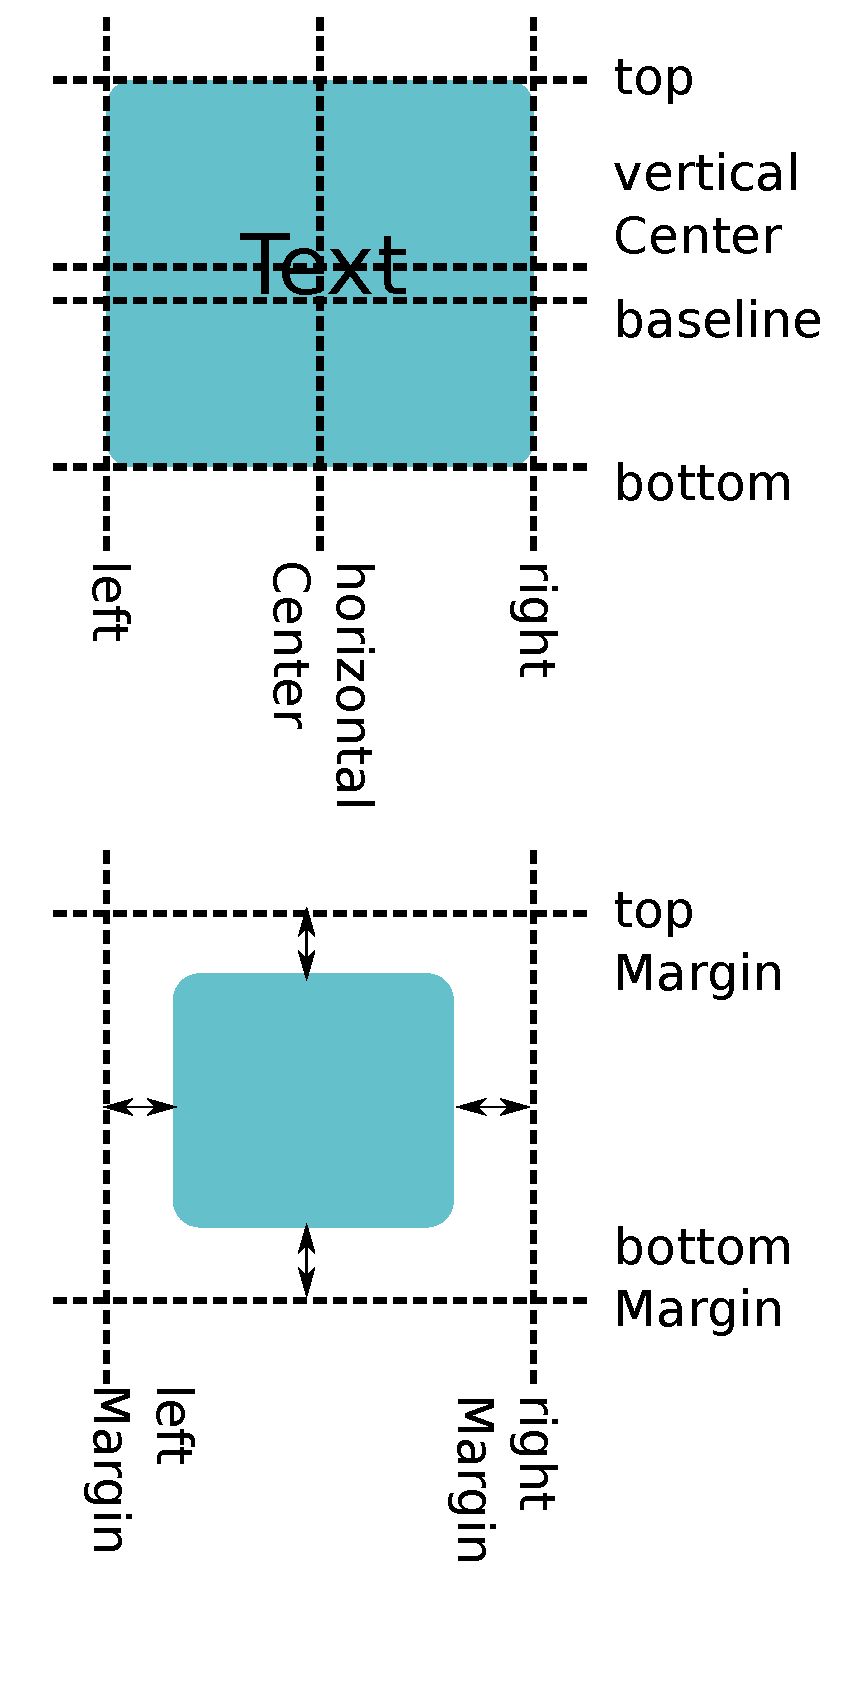
\includegraphics[width=\textwidth]{images/anchors.pdf}
      \end{figure}
    \end{column}
  \end{columns}
\end{frame}

\begin{frame}[fragile]
  \frametitle{Qt Quick -- anchoring examples}
    \footnotesize
    \begin{columns}
      \begin{column}{0.55\textwidth}
      \begin{itemize}
        \item \verb@rect2@ right of \verb@rect1@
        \begin{lstlisting}[basicstyle=\scriptsize\ttfamily]
	Rectangle {
	  id: rect1; ...
	}
	Rectangle {
	  id: rect2; ...
	  anchors.left: rect1.right;
	}
        \end{lstlisting}
        \item \verb@rect2@ bottom right of \verb@rect1@
        \begin{lstlisting}[basicstyle=\scriptsize\ttfamily]
	Rectangle {
	  id: rect1; ...
	}
	Rectangle {
	  id: rect2; ...
	  anchors.left: rect1.right;
	  anchors.top: rect1.bottom;
	}
        \end{lstlisting}
      \end{itemize}
      \end{column}
      \begin{column}{0.45\textwidth}
      \begin{itemize}
        \item \verb@Text@ horizontally centered within its visual parent,
          with fixed vertical position
        \begin{lstlisting}[basicstyle=\tiny\ttfamily]
	Window {
	  width: 320;
	  height: 130;
	  ...

	  Text {
	    text: "My text item"

	    anchors.horizontalCenter:
	      parent.horizontalCenter;
	    y: 40;
	    ...
	  }
	}
        \end{lstlisting}
      \end{itemize}
      \end{column}
    \end{columns}
\end{frame}

\begin{frame}[fragile]
  \frametitle{Qt Quick -- item positioners}
    \footnotesize
    \begin{columns}
      \begin{column}{0.55\textwidth}
      \begin{itemize}
        \item Container items which manage the positions of items in
          a declarative user interface.
        \item Similar to the widget layouts, except that they {\em are} containers.
      \end{itemize}
      \rowcolors{2}{green!80!yellow!50}{green!70!yellow!40}
      \scriptsize
      \begin{tabular}{|p{0.2\textwidth}|p{0.7\textwidth}|}
        \hline
        \textbf{Positioner} & \textbf{Description} \\
        \hline
        Column & Positions children in a column \\
        \hline
        Row & Positions children in a row \\
        \hline
        Flow & Positions children in a row, wrapping as necessary \\
        \hline
        Grid & Positions its children in a grid \\
        \hline
        Layout\-Mirroring & Property used to mirror layout behavior \\
        \hline
      \end{tabular}
      \end{column}
      \begin{column}{0.45\textwidth}
      \begin{itemize}
        \item 
        \begin{lstlisting}[basicstyle=\tiny\ttfamily]
	Item {
	width: 310; height: 170

	  Column {
	    anchors.horizontalCenter:
	      parent.horizontalCenter;
	    anchors.verticalCenter:
	      parent.verticalCenter;

	    spacing: 5

	    Rectangle { ... }
	    Rectangle { ... }
	    Rectangle { ... }

	    Text { ... }
	  }
	}
        \end{lstlisting}
      \end{itemize}
      \end{column}
    \end{columns}
\end{frame}

\begin{frame}
  \frametitle{Qt Quick -- States, Transitions and Animations\footnote
    {\url{doc.qt.io/qt-5.6/qtquick-statesanimations-topic.html}}}
  \small
  \begin{itemize}
    \item Animating between various user interface states can be beneficial
      to the user experience.
    \item Qt Quick provides objects representing the states and changes
      of visual elements:
      \begin{itemize}
        \item States
        \begin{itemize}
          \item Encapsulate particular sets of settings of properties 
          for a visual elements.
          \item Can be hierarchical.
        \end{itemize}
        \item Transitions
        \begin{itemize}
          \item Allow simple smooth transitions between two states, instead
            of abrupt changes.
          \item Use basic interpolation methods.
        \end{itemize}
        \item Behaviors, Animations and Animators
        \begin{itemize}
          \item Allow complex and customizable animations of various item
            properties.
        \end{itemize}
      \end{itemize}
  \end{itemize}
\end{frame}

\begin{frame}
  \frametitle{Qt Quick -- user interaction}
  \begin{itemize}
    \item Depending on the application deployment platform or particular device
      various types of user input can be used in QML applications:
      \begin{itemize}
        \item Mouse -- \texttt{MouseArea}, \texttt{MouseEvent}
        \item Touch-screen -- \texttt{Flickable}, \texttt{MultiPointTouchArea}
        \item Keyboard -- \texttt{Keys}
        \item Device motion sensors -- accelerometer, camera, GPS, thermometers,
          etc., provided by the {\em Qt Sensors}\footnote
          {\url{http://doc.qt.io/qt-5.6/qtsensors-index.html}} module.
      \end{itemize}
      \item Qt signals and slots are used to deliver input interactions.
  \end{itemize}
\end{frame}

\begin{frame}[fragile]
  \frametitle{Qt Quick -- \texttt{MouseArea}\footnote
    {\url{http://doc.qt.io/qt-5.6/qml-qtquick-mousearea.html}}}
  \begin{columns}
    \begin{column}{0.5\textwidth}
    \begin{itemize}
      \item Captures the following mouse interaction events:
      \begin{itemize}
        \small
        \item canceled
        \item clicked
        \item doubleClicked
        \item entered
        \item exited
        \item positionChanged
        \item pressAndHold
        \item pressed
        \item released
      \end{itemize}
    \end{itemize}
    \end{column}
    \begin{column}{0.5\textwidth}
      \begin{lstlisting}[basicstyle=\tiny\ttfamily]
	Window {
	  width: 320; height: 130
	  color: "lightgreen"

	  Text { ... }

	  Text {
	    text: "Close"
	    anchors.bottom:
	      parent.baseline;
	    anchors.horizontalCenter:
	      parent.horizontalCenter;
	    font.pointSize: 12

	    MouseArea {
	      anchors.fill: parent
	      onClicked: Qt.quit()
	    }
	  }
	}
      \end{lstlisting}
    \end{column}
  \end{columns}
\end{frame}

\begin{frame}[fragile]
  \frametitle{Qt Quick -- \texttt{Keys}\footnote
    {\url{http://doc.qt.io/qt-5.6/qml-qtquick-keys.html}}}
  \begin{columns}
    \footnotesize
    \begin{column}{0.55\textwidth}
    \begin{itemize}
      \item Implements key press handling functionality
      \item Visual items have the \texttt{Keys} attached property to enable
        key events.
      \item Keyboard events are generally handled in two signal properties:
      \begin{itemize}
        \scriptsize
        \item pressed
        \item released
      \end{itemize}
      \item Special keys have their own signal handlers:
      \begin{itemize}
        \scriptsize
        \item noPressed
        \item yesPressed
        \item upPressed
        \item downPressed
        \item leftPressed
        \item rightPressed
        \item \ldots
      \end{itemize}
    \end{itemize}
    \end{column}
    \begin{column}{0.45\textwidth}
      \begin{lstlisting}[basicstyle=\tiny\ttfamily]
	Rectangle {
	  anchors.fill: parent
	  focus: true

	  Keys.onUpPressed: {
	    console.log("move up");
	    event.accepted = true;
	  }

	  Keys.onDownPressed: {
	    console.log("move down");
	    event.accepted = true;
	  }

	  Keys.onPressed: {

	    if (event.key == Qt.Key_Left) {

	      console.log("move left");
	      event.accepted = true;
	    }
	    if (event.key == Qt.Key_Right) {

	      console.log("move right");
	      event.accepted = true;
	    }
	  }
	}
      \end{lstlisting}
    \end{column}
  \end{columns}
\end{frame}

\begin{frame}
  \frametitle{Qt Quick -- controls\footnote
    {\url{http://doc.qt.io/qt-5.6/qtquickcontrols-index.html}} -- Main window}
  \rowcolors{2}{green!80!yellow!50}{green!70!yellow!40}
  \begin{tabular}{|p{0.3\textwidth}|p{0.6\textwidth}|}
        \hline
        \textbf{Control} & \textbf{Description} \\
        \hline
        Action & Abstract user interface action that can be bound to items \\
        \hline
        ApplicationWindow & Provides a top-level application window \\
        \hline
        MenuBar & Provides a horizontal menu bar \\
        \hline
        StatusBar & Contains status information in your app \\
        \hline
        ToolBar & Contains ToolButton and related controls \\
        \hline
  \end{tabular}
\end{frame}

\begin{frame}
  \frametitle{Qt Quick -- controls\footnote
    {\url{http://doc.qt.io/qt-5.6/qtquickcontrols-index.html}} -- Navigation and views}
  \rowcolors{2}{green!80!yellow!50}{green!70!yellow!40}
  \begin{tabular}{|p{0.2\textwidth}|p{0.7\textwidth}|}
        \hline
        \textbf{Control} & \textbf{Description} \\
        \hline
        ScrollView & Provides a scrolling view within another Item \\
        \hline
        SplitView & Lays out items with a draggable splitter between each item \\
        \hline
        StackView & Provides a stack-based navigation model \\
        \hline
        TabView & A control that allows the user to select one of multiple stacked items \\
        \hline
        TableView & Provides a list view with scroll bars, styling and header sections \\
        \hline
        TreeView & Provides a tree view with scroll bars, styling and header sections \\
        \hline
  \end{tabular}
\end{frame}

\begin{frame}
  \frametitle{Qt Quick -- controls\footnote
    {\url{http://doc.qt.io/qt-5.6/qtquickcontrols-index.html}} -- Common}
  \rowcolors{2}{green!80!yellow!50}{green!70!yellow!40}
  \footnotesize
  \begin{tabular}{|p{0.2\textwidth}|p{0.7\textwidth}|}
        \hline
        \textbf{Control} & \textbf{Description} \\
        \hline
        Button & A push button with a text label \\
        \hline
        CheckBox & A checkbox with a text label \\
        \hline
        ComboBox & Provides a drop-down list functionality \\
        \hline
        GroupBox & Group box frame with a title \\
        \hline
        Label & A text label \\
        \hline
        Menu & Provides a menu component for use as a context menu, popup menu,
          or as part of a menu bar \\
        \hline
        ProgressBar & A progress indicator \\
        \hline
        Slider & Provides a vertical or horizontal slider control \\
        \hline
        SpinBox & Provides a spin box control \\
        \hline
        StatusBar & Contains status information in your app \\
        \hline
        Switch & A switch \\
        \hline
	TextArea & Displays multiple lines of editable formatted text \\
        \hline
	TextField & Displays a single line of editable plain text \\
        \hline
	ToolBar & Contains ToolButton and related controls \\
        \hline
  \end{tabular}
\end{frame}

 \begin{frame}[fragile]
  \frametitle{Qt QML\footnote{\url{http://doc.qt.io/qt-5.6/qtqml-index.html}}}
  \small
  \begin{itemize}
    \item Defines and implements the QML language and engine infrastructure.
    \item Implements commonly used QML types.
    \item Framework for developing applications and libraries using the QML
      language. 
    \item Framework for running JavaScript expressions in QML and from C++.
    \item Using from C++
    \begin{itemize}
      \item \verb@#include <QtQml>@
    \end{itemize}
    \item Using from QML
    \begin{itemize}
      \item \verb@import QtQml 2.0@
    \end{itemize}
    \item Project files
    \begin{itemize}
      \item \verb@QT += qml@
    \end{itemize}
  \end{itemize}
\end{frame}

 \begin{frame}[fragile]
  \frametitle{Integration with C++ -- simple Qt Quick application}
  \begin{lstlisting}
	#include <QtCore>
	#include <QGuiApplication>
	#include <QQuickView>
	#include <QUrl>

	int main(int argc, char** argv)
	{
	    QGuiApplication app(argc, argv);
	    QQuickView qmlview(QUrl("qrc:///semaphore.qml"));
	    qmlview.show();
	    return app.exec();
	}
  \end{lstlisting}
\end{frame}

 \begin{frame}[fragile]
  \frametitle{Integration with C++ -- QML resources}
  \begin{lstlisting}
	<!DOCTYPE RCC><RCC version="1.0">
	<qresource>
	    <file>SemLight.qml</file>
	    <file>semaphore.qml</file>
	    <file>stop.svg</file>
	    <file>walk.svg</file>
	</qresource>
	</RCC>
  \end{lstlisting}
\end{frame}

 \begin{frame}[fragile]
  \frametitle{Integration with C++ -- Implementing QML object}
  \begin{lstlisting}[basicstyle=\scriptsize\ttfamily]
	class SemManager
 	 : public QObject
	{
	    Q_OBJECT
	    Q_PROPERTY(QString semState
	               READ getSemState
	               NOTIFY semStateChanged
	    )

	    bool _stop;
	public:
	    SemManager(QObject* parent = 0);

	    QString getSemState(void) const;
	signals:
	    void semStateChanged(void);
	public slots:
	    void activate(void);
	    void stop(void);
	    void go(void);
	};
  \end{lstlisting}
\end{frame}

 \begin{frame}[fragile]
  \frametitle{Integration with C++ -- Using custom QML object}
  \begin{itemize}
  \item Registering in C++
  \begin{lstlisting}[basicstyle=\scriptsize\ttfamily]
	qmlRegisterType<SemManager>(
	    "sk.uniza.fri.qt",
	    1, 0,
	    "SemManager"
	);
  \end{lstlisting}
  \item Importing in QML
  \begin{lstlisting}[basicstyle=\scriptsize\ttfamily]
	import sk.uniza.fri.qt 1.0
  \end{lstlisting}
  \item Using in QML
  \begin{lstlisting}[basicstyle=\scriptsize\ttfamily]
	SemManager { id: "manager" }

	MouseArea {
	    anchors.fill: parent
	    onClicked: manager.activate()
	}
  \end{lstlisting}
  \end{itemize}
\end{frame}

 \begin{frame}[fragile]
  \frametitle{Integration with C++ -- Qt Quick controls application}
  \begin{lstlisting}[basicstyle=\scriptsize\ttfamily]
	#include <QtCore>
	#include <QGuiApplication>
	#include <QQmlApplicationEngine>
	#include <QQuickView>
	#include <QtQml>
	#include <QUrl>

	int main(int argc, char** argv)
	{
	    QGuiApplication app(argc, argv);

	    QQmlApplicationEngine engine;
	    engine.load(QUrl("qrc:///main.qml"));

	    QObject* root = engine.rootObjects().value(0);
	    QQuickWindow* win = qobject_cast<QQuickWindow*>(root);
	    win->show();

	    return app.exec();
	}
  \end{lstlisting}
\end{frame}

